%------------------------------------------------------------------------------
\subsection{Installateur logiciel}
\begin{frame}\frametitle{Déploiement d'une application}
\begin{itemize}
 \item Déploiement de l'application sur une machine
 \item Procédures d'installation parfois lourdes
 \item Procédures délicates
\end{itemize}
\end{frame}
%------------------------------------------------------------------------------
\begin{frame}[fragile]\frametitle{Installation de Glassfish}

\centering

\includegraphics[width=.3\linewidth]{../image/glassfishLogo.png}
\vfill
\begin{beamerboxesrounded}[shadow=true]{Proc\'edure d'installation de Glassfish-v2}
	
	\begin{verbatim}
	java -Xmx256m -jar glassfish-installer-v2.1.jar;
	cd glassfish;
	chmod -R +x lib/ant/bin;
	lib/ant/bin/ant -f setup.xml;
	bin/asadmin start-domain;
	\end{verbatim}
\end{beamerboxesrounded}
\end{frame}
%------------------------------------------------------------------------------
\begin{frame}\frametitle{Installateur logiciel}
\begin{beamerboxesrounded}[shadow=true]{But}
 \begin{itemize}
  \item Automatiser les procédures d'installation
  \item Assurer une intégration dans le système
  \item Assister l'utilisateur
 \end{itemize}
\end{beamerboxesrounded}
\vfill
\begin{beamerboxesrounded}[shadow=true]{Inconvénients}
 \begin{itemize}
  \item Dépendant de l'OS
  \item Création de l'interface graphique lourde
 \end{itemize}
\end{beamerboxesrounded}
\end{frame}
%------------------------------------------------------------------------------
\subsection{IzPack}
\begin{frame}\frametitle{IzPack}
\begin{minipage}[c]{.46\linewidth}
	\begin{beamerboxesrounded}[shadow=true]{But}
		\begin{itemize}
		\item Déporter la création l'installateur
		\end{itemize}
	\end{beamerboxesrounded}
\end{minipage}
\hfill
\begin{minipage}[c]{.46\linewidth}
	\begin{beamerboxesrounded}[shadow=true]{Multiplateforme}
		\begin{itemize}
		\item Java 1.5
		\item Windows, Mac, BSD, Linux...
		\end{itemize}
	\end{beamerboxesrounded}
\end{minipage}
\vfill
\begin{minipage}[c]{.46\linewidth}
	\begin{beamerboxesrounded}[shadow=true]{Personnalisable}
		\begin{itemize}
		\item Descripteur XML
		\item Contrôle l'aspect et la logique
		\end{itemize}
	\end{beamerboxesrounded}
\end{minipage}
\hfill
\begin{minipage}[c]{.46\linewidth}
	\begin{beamerboxesrounded}[shadow=true]{Open-Source}
		\begin{itemize}
		\item License Apache 2
		\item Projet Membre de Codehaus
		\end{itemize}
	\end{beamerboxesrounded}
\end{minipage}
\end{frame}
%------------------------------------------------------------------------------
\begin{frame}\frametitle{Principe d'IzPack}
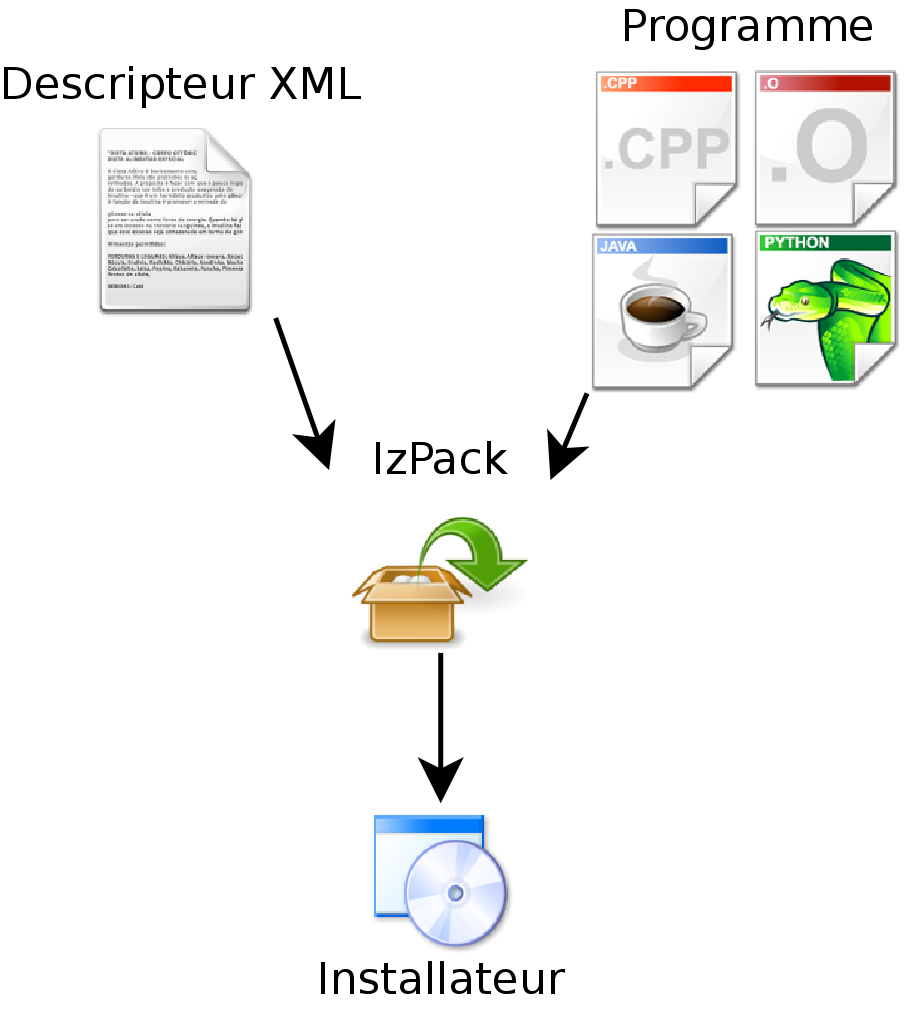
\includegraphics[width=1\linewidth]{../image/izpackInstall.png}
\end{frame}
%------------------------------------------------------------------------------
\subsection{Problèmes}
\begin{frame}\frametitle{Problèmes}
	\begin{beamerboxesrounded}[shadow=true]{NanoXML obsolète}
		\begin{itemize}
		\item Bugs connus
		\item Fonctionnalités manquantes
		\item Développement arrêté
		\end{itemize}
	\end{beamerboxesrounded}
	\vfill
	\begin{beamerboxesrounded}[shadow=true]{Conséquences}
		\begin{itemize}
			\item Invisibles pour l'utilisateur
			\item Génantes pour le développeur	
		\end{itemize}
	\end{beamerboxesrounded}
\end{frame}
%------------------------------------------------------------------------------
\begin{frame}\frametitle{Problèmes}
\begin{itemize}
	\item Comment supprimer NanoXML?
	\item Par quoi le remplacer?
\end{itemize}
\end{frame}
%------------------------------------------------------------------------------
